\documentclass[sigconf]{acmart}
% \documentclass[conference]{IEEEtran}
% \documentclass[12pt]{article}

\usepackage{lipsum}
\usepackage{graphicx}
\usepackage{algorithmic}
% \usepackage{cite}
% \usepackage{amsmath,amssymb,amsfonts}
% \usepackage{textcomp}
% \usepackage{xcolor}

% \def\BibTeX{{
%   \rm B\kern-.05em{\sc i\kern-.025em b}\kern-.08em
%   T\kern-.1667em\lower.7ex\hbox{E}\kern-.125emX
% }}

% \BibTeX command to typeset BibTeX logo in the docs
\AtBeginDocument{%
  \providecommand\BibTeX{{%
    \normalfont B\kern-0.5em{\scshape i\kern-0.25em b}\kern-0.8em\TeX
  }}
}

%% Rights management information.  This information is sent to you
%% when you complete the rights form.  These commands have SAMPLE
%% values in them; it is your responsibility as an author to replace
%% the commands and values with those provided to you when you
%% complete the rights form.
\setcopyright{acmcopyright}
\copyrightyear{2018}
\acmYear{2018}
\acmDOI{10.1145/1122445.1122456}

%% These commands are for a PROCEEDINGS abstract or paper.
% \acmConference[Woodstock '18]{Woodstock '18: ACM Symposium on Neural
%   Gaze Detection}{June 03--05, 2018}{Woodstock, NY}
\acmBooktitle{Woodstock '18: ACM Symposium on Neural Gaze Detection,
  June 03--05, 2018, Woodstock, NY}
\acmPrice{15.00}
\acmISBN{978-1-4503-XXXX-X/18/06}

% \author{
%   \IEEEauthorblockN{1\textsuperscript{st} Alisamar Husain}
%   \IEEEauthorblockA{
%     \textit{Jamia Millia Islamia University}\\
%     New Delhi, India\\
%   }
%   \and
%   \IEEEauthorblockN{2\textsuperscript{nd}Alisamar Husain}
%   \IEEEauthorblockA{
%     \textit{Jamia Millia Islamia University}\\
%     New Delhi, India\\
%     syed176412@st.jmi.ac.in
%   }
% }

\begin{document}
  \title{CryptoGAN: An Approach to Neural Cryptography}

  \author{Alisamar Husain}
  \email{syed176412@st.jmi.ac.in}
  \affiliation{
    \institution{Jamia Millia Islamia University}
    \streetaddress{Maulana Mohammad Ali Jauhar Marg}
    \city{New Delhi}
    \state{Delhi}
    \postcode{110025}
  }

  \begin{abstract}
    \lipsum[1]
  \end{abstract}
  
  \keywords{datasets, neural networks, gaze detection, text tagging}
  \begin{teaserfigure}
    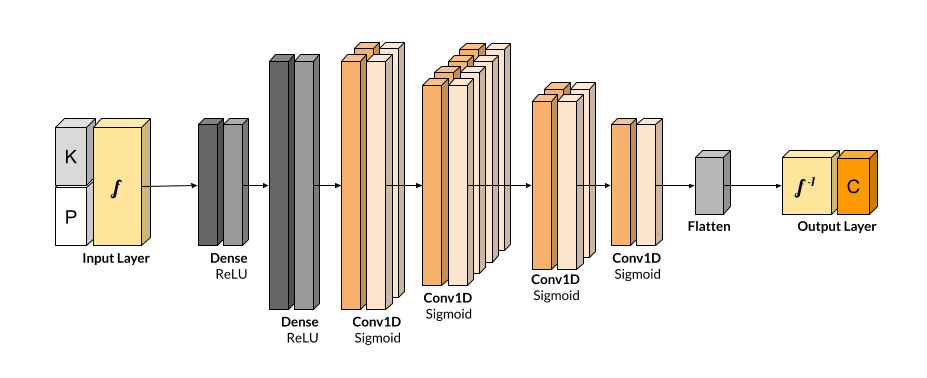
\includegraphics[width=\textwidth]{ref/netmodel}
    \caption{Network Model from Coutinho et al.}
    \label{fig:teaser}
  \end{teaserfigure}

  \maketitle
 
  \section{Introduction}
  This is my tiny Introduction with a nice 
  little citation \cite{visualloss}

  This is my tiny Introduction with a nice 
  little citation \cite{seminalanc}
  
  % This is my tiny Introduction with a nice 
  % little citation \cite{netsync}
  
  This is my tiny Introduction with a nice 
  little citation \cite{perfanc}

  \section{Methodology} 
  \lipsum
  
  \bibliographystyle{ACM-Reference-Format}
  \bibliography{../resources/citations}
\end{document}
